\let\negmedspace\undefined
\let\negthickspace\undefined
\documentclass[journal,12pt,twocolumn]{IEEEtran}
\usepackage{cite}
\usepackage{amsmath,amssymb,amsfonts,amsthm}
\usepackage{algorithmic}
\usepackage{graphicx}
\usepackage{textcomp}
\usepackage{xcolor}
\usepackage{txfonts}
\usepackage{listings}
\usepackage{enumitem}
\usepackage{mathtools}
\usepackage{gensymb}
\usepackage{comment}
\usepackage[breaklinks=true]{hyperref}
\usepackage{tkz-euclide} 
\usepackage{listings}
\usepackage{gvv}                                        
\def\inputGnumericTable{}                                 
\usepackage[latin1]{inputenc}                                
\usepackage{color}                                            
\usepackage{array}                                            
\usepackage{longtable}                                       
\usepackage{calc}                                             
\usepackage{multirow}                                         
\usepackage{hhline}                                           
\usepackage{ifthen}                                           
\usepackage{lscape}

\newtheorem{theorem}{Theorem}[section]
\newtheorem{problem}{Problem}
\newtheorem{proposition}{Proposition}[section]
\newtheorem{lemma}{Lemma}[section]
\newtheorem{corollary}[theorem]{Corollary}
\newtheorem{example}{Example}[section]
\newtheorem{definition}[problem]{Definition}
\newcommand{\BEQA}{\begin{eqnarray}}
\newcommand{\EEQA}{\end{eqnarray}}
\newcommand{\define}{\stackrel{\triangle}{=}}
\theoremstyle{remark}
\newtheorem{rem}{Remark}

\usepackage{graphicx}
\graphicspath{ {./Downloads/} }
\begin{document}

\bibliographystyle{IEEEtran}
\vspace{3cm}

\title{GATE 2023}
\author{EE22BTECH11060 - TEJAVATH KUSHAL$^{*}$% <-this % stops a space
}
\maketitle
\newpage
\bigskip

\renewcommand{\thefigure}{\theenumi}
\renewcommand{\thetable}{\theenumi}

\maketitle
\noindent \textbf{Q 20 :} The solution \(x(t)\), \(t \geq 0\), to the differential equation
$\ddot{x} = -k\dot{x} , k > 0$
with initial conditions \(x(0) = 1\) and \(\dot{x} (0) = 0\) is: \quad \brak{GATE ~2023  , IN} \\

\noindent \textbf{Ans}:\\ \\
\begin{table}[h]
\centering
\begin{tabular}{ | c | c|  } 
  \hline
   Differential equation & $\ddot{x} = -k\dot{x}$ \\ 
  \hline
  Initial conditions & $x\brak{})=1$ and $\dot{x}\brak{0}=0$ \\
  \hline
  $x\brak{t}$ & $?$ \\ 
  \hline
\end{tabular}
\caption{Parameter Table}
\label{tab:gate2023.in.20}
\end{table}
\begin{align}
    \implies \frac{d^2 x(t)}{dt^2} = -k\frac{dx(t)}{dt}
\end{align}\\

Taking Laplace transform on both sides,\\
\begin{align}
\label{eq:gate2023.in.20.2}\frac{d^2x\brak{t}}{dx^2} &\system{L}
       s^2X(s)-sx(0)-\dot{x}(0)\\
\label{eq:gate2023.in.20.3}\frac{dx\brak{t}}{dx} &\system{L} sX(s)-x(0)
\end{align}

From Table \eqref{eq:gate2023.in.20.2} , \eqref{eq:gate2023.in.20.3} 
\begin{align}
s^2 X\brak{s} - sx\brak{0} - \dot{x}\brak{0} &= -k\brak{sX\brak{s} - x\brak{0}} \\
s^2 X\brak{s} - s &= -k\brak{sX\brak{s}-1} \\
sX\brak{s}\brak{s+k}&=\brak{s+k}\\
     \notag s &\neq -k\\
     X\brak{s}&=\frac{1}{s}  \\
     x\brak{t}&=u\brak{t}\\
      \implies x\brak{t}&=1 \quad \brak{t\geq 0}
\end{align}\\
\pagebreak
\begin{figure}[h]
    %\caption{ Plot of $x\brak{t}$ v/s t}
    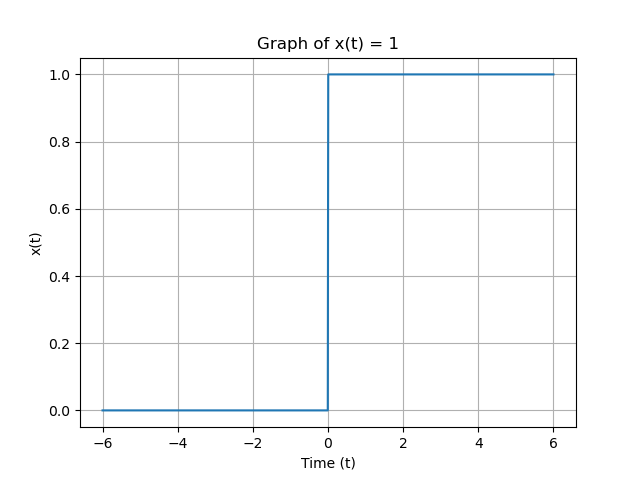
\includegraphics[width=0.5\textwidth]{figs/x(t)_vs_t.png}\label{fig:plot}
    \caption{Plot of $x\brak{t}$ v/s t}
\end{figure}



\end{document}
